\documentclass{article}
\usepackage[letterpaper, left=2.5cm, right=2.5cm, top=2.5cm, bottom=2.5cm]{geometry}
\usepackage{graphicx}
\usepackage{epstopdf}
\usepackage{fge}
\begin{document}

\title{PAL Compiler Documentation }
\date{\today}
\author{Chris Pavlicek, Connor Moreside, Mike Armstrong, and Steve Jahns}
\maketitle

% From checkpoint 1 spec:
%
% Documentation
%
% Your documentation should describe what your group has done on the
% project. This does not mean that you should reiterate class notes; I want to
% know what is different about your group. Some things you may want to discuss
% include: handling of lexical units, syntax error reporting strategies, syntax
% error recovery (if any) , problems encountered and their solutions, etc.
% When writing, remember who is going to read it—skip the preli minaries
% and get to the point. There is a page limit of 12 double-spaced pages,
% not in cluding diagrams.

\section*{Overview}

\begin{figure}[h!]
\centering 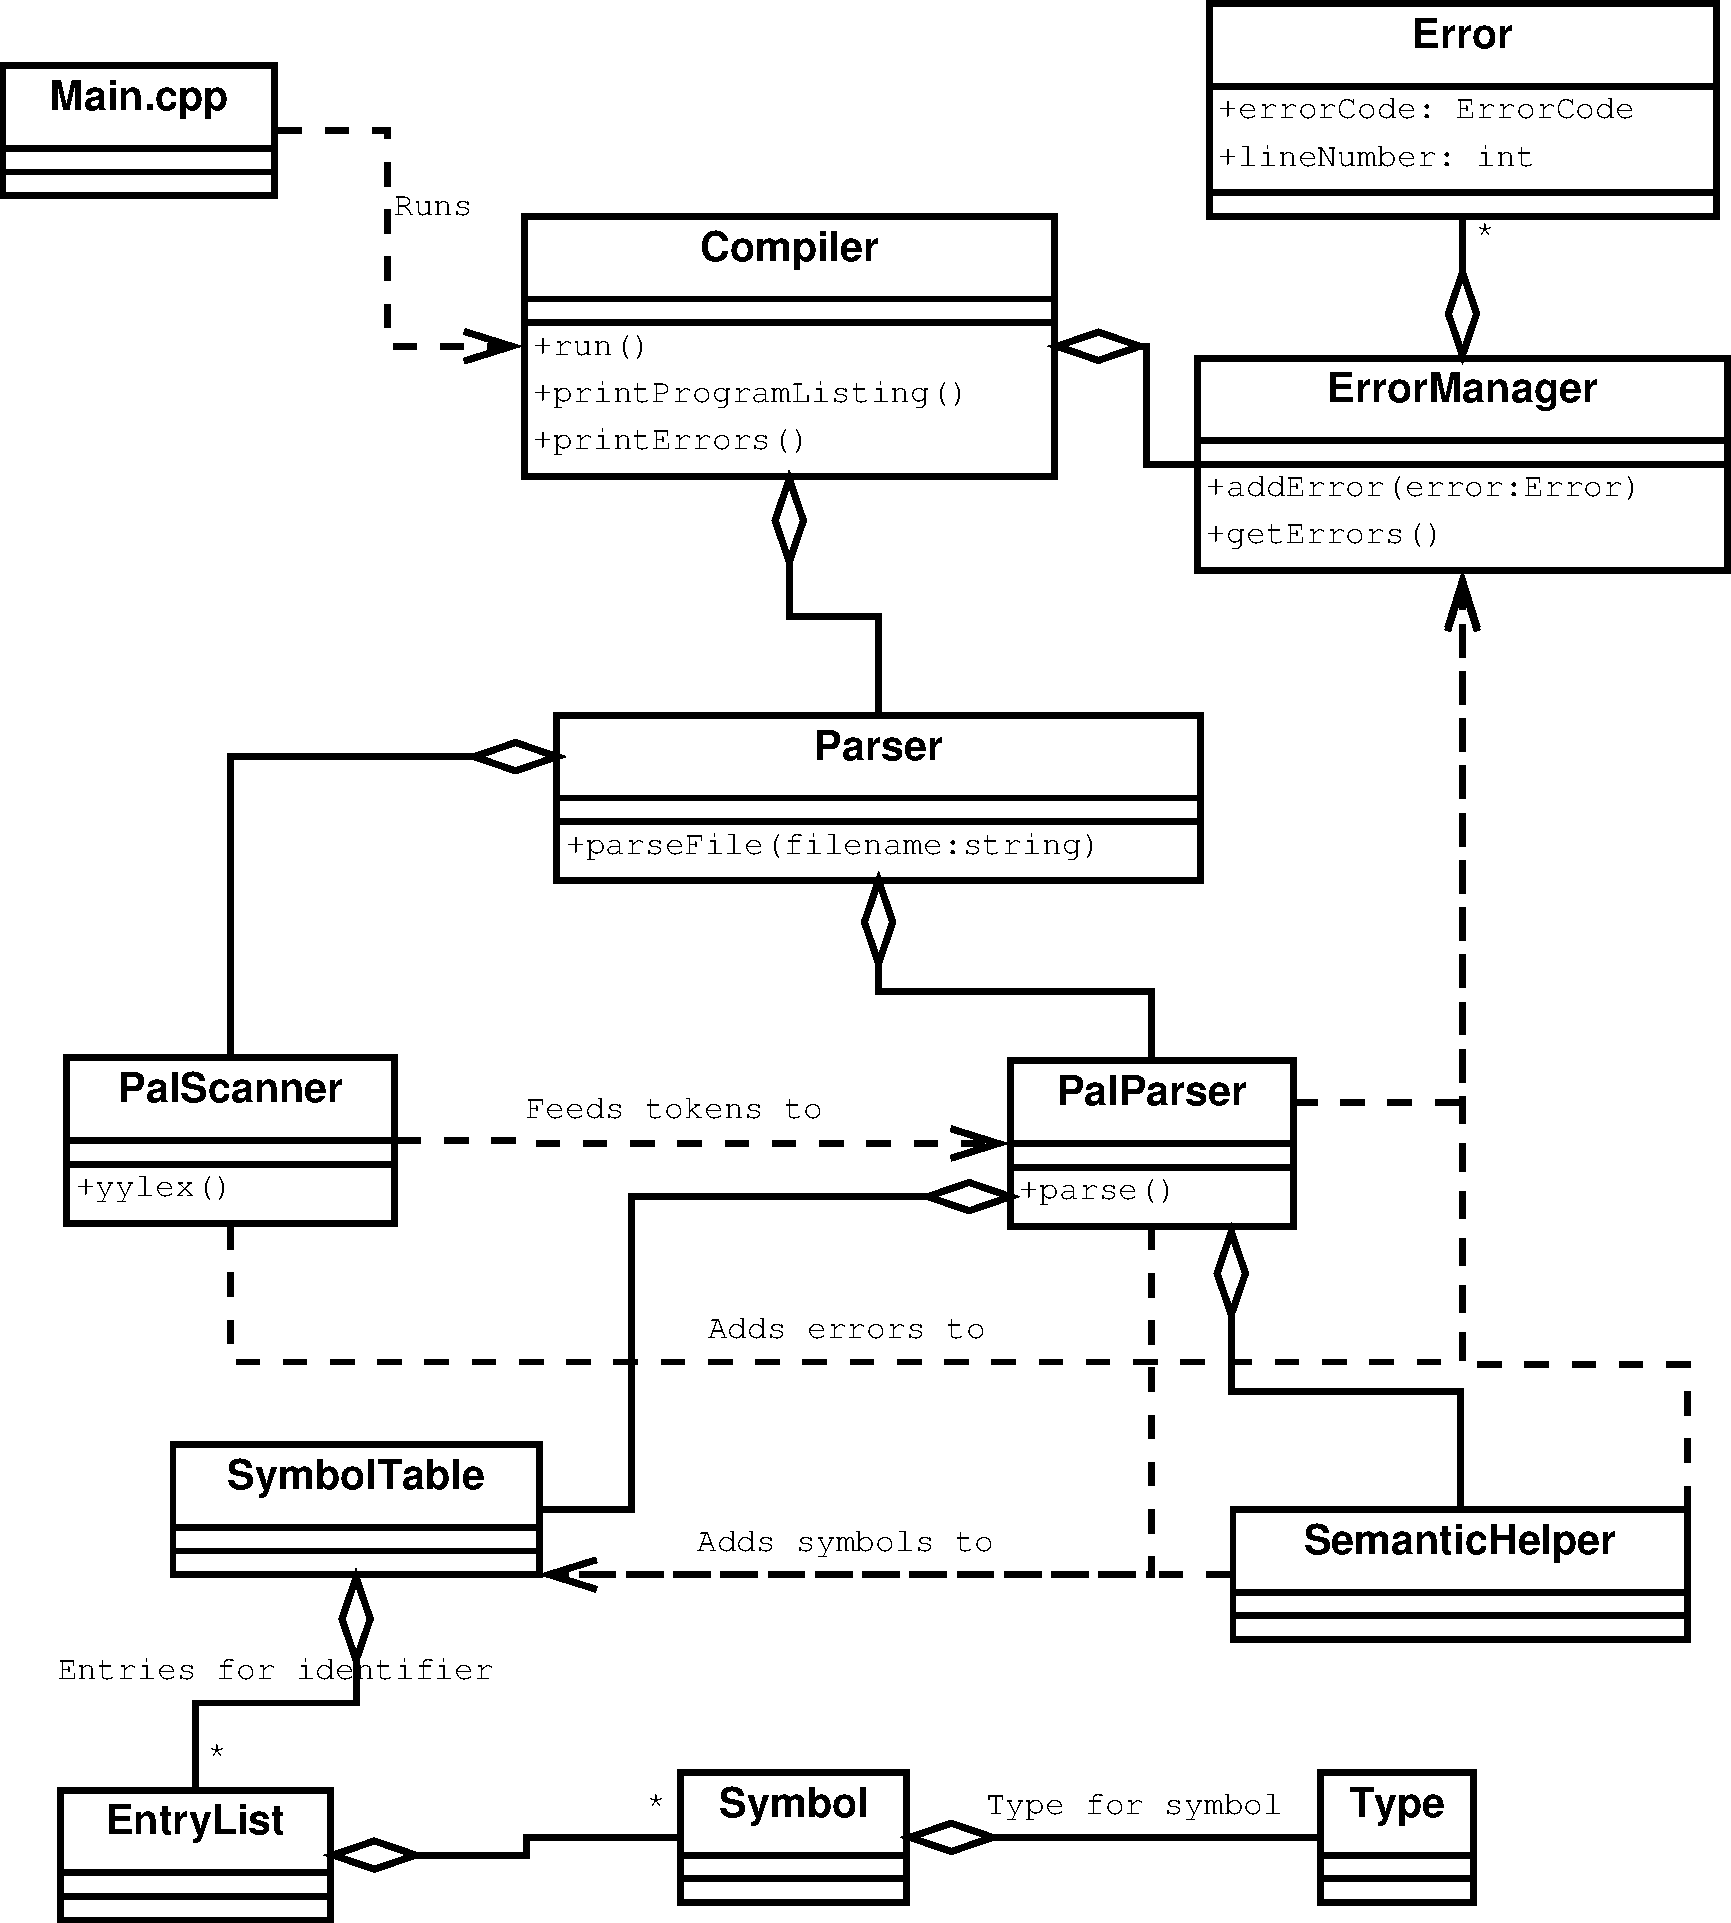
\includegraphics[width=10cm]{uml.pdf}
\caption{General structure of the compiler's parsing components.}
\end{figure}

At this stage, our compiler source consists of 6 classes. The \texttt{Compiler} class is instantiated by 
the program's \texttt{main()} function, and ran with the program's given command line arguments. 

The \texttt{Compiler} class creates an \texttt{ErrorManager}
class which tracks errors as they are detected while parsing the file. It passes the \texttt{ErrorManager}
to the \texttt{Parser} class when it is constructed.

The \texttt{Parser} class is a wrapper for the \texttt{flex} and \texttt{bison}
generated \texttt{PalScanner} and \texttt{PalParser} classes, from the
\texttt{pal.lex} and \texttt{pal.y} sources, respectively. \texttt{Parser}
parses a file with \texttt{parseFile(fileName)}, which creates a
\texttt{PalScanner} and \texttt{PalParser} where the scanner runs through
the file and feeds the parser with a stream of tokens.  The scanner and
parser are given access to the common \texttt{ErrorManager}, and when they
encounter errors during lexical and syntactical analysis, they create new
\texttt{Error} objects with the appropriate error code and line number and
give them to the \texttt{ErrorManager}.

When parsing is finished, the \texttt{Compiler} takes the errors accumulated by
the \texttt{ErrorManager} and either displays them inline with the program
listing, or all errors in order of appearance without the program listing if 
\texttt{pal} was invoked with the \texttt{-n} option.

	% Overall design
	% Outline of classes + dependencies

\section*{Lexical Analysis}

Our lexical analyser is generated by GNU Flex from the source in \texttt{./src/pal.lex}, which
is bundled into the \texttt{PalScanner} class. It is capable of recognizing the following
errors at the lexical level:

\begin{description}
  \item[Unclosed Comment]
	  If a comment is started with \texttt{\{} but is not followed by a
	  \texttt{\}} later in the file, the scanner will report an error.  In
	  our scanner, the comment rule will match to the end of the file in
	  this situation, so unfortunately no more analysis of the file is
	  possible at this point.
	  % TODO should we consider backtracking to the next line somehow?

  \item[Unexpected Comment End]
	  If the scanner encounters a \texttt{\}} when it is not in a comment,
	  it will report an error. Otherwise, the extra brace is ignored and analysis 
	  continues in an attempt to find more errors in the file.

  \item[Multi-line String Literal]
	  % TODO make sure this is actually implemented!
	  In the PAL language, a string literal cannot span multiple lines, so 
	  if the scanner encounters a string literal that extends beyond the next
	  newline, it will report an error that indicates the start and finish line
	  of the illegal multi-line string. It will still return a \texttt{STRING\_LITERAL}
	  token, and continue analysis to try and find more errors.

  \item[Invalid Character or Escaped Character in String]
	  The scanner will report an invalid character/escaped character in a string
	  literal if it contains either of the following:
	  \begin{itemize}
		  \item a \texttt{\textbackslash} that is not followed by a 
			  \texttt{'}, \texttt{n}, or \texttt{t}
		  \item a \texttt{\textbackslash} at the end of the string, that
			  is not preceded by another \texttt{\textbackslash}
	  \end{itemize}

	  % TODO would be cool if it actually printed the invalid character!

	% TODO \ at end of string? what kind of error? test!?

  \item[Invalid Identifier]
	  Valid PAL identifiers start with at least one letter, followed by any number
	  of letters or numbers. Identifiers that start with numbers will be reported
	  as an error. 
	% TODO can we detect other invalid identifiers?

\end{description}

\section*{Syntax Analysis}

	% TODO
	% handling of lexical units
	% syntax error reporting
	% recovery strategies

\section*{Testing}
	% TODO
	% gtest, unit tests
	% whole file tests

% known bugs?
% extra features?

\end{document}
